<<<<<<< HEAD
 
=======

>>>>>>> counterfactuals

\documentclass{beamer}

\usepackage{amsthm,amssymb,amsmath}
\usepackage[round]{natbib}
\bibliographystyle{asa}
\usepackage{amsmath}
\usepackage{amsfonts}
\usepackage{amssymb}
\usepackage{amsthm}


\usepackage[normalem]{ulem}
\usepackage{booktabs}

\usepackage{calc,tikz,nicefrac}
\usetikzlibrary{positioning}
%\geometry{letterpaper}
%\usepackage{xcolor}
%\usepackage[usenames, dvipsnames]{color}

\def\mb{\mathbf}
\def\iid{\mathrm{i.i.d. }}
\def\bs{\boldsymbol}

\mode<presentation>
{
  \usetheme{metropolis}
%  \usetheme{Boadilla}
  %\usetheme{Warsaw}
  % or ...

  \setbeamercovered{transparent}
  % or whatever (possibly just delete it)
}

\def\mb{\mathbf}
\def\iid{\mathrm{i.i.d. }}
\def\bs{\boldsymbol}
\def\tbf{\textbf}
\def\t{^{\top}}
\def\bSig{\bs{\Sigma}}
\newcommand{\mcitet}[1]{\mbox{\citet{#1}}}
<<<<<<< HEAD
\newcommand{\mcitep}[1]{\mbox{\citep{#1}}} 
=======
\newcommand{\mcitep}[1]{\mbox{\citep{#1}}}
>>>>>>> counterfactuals

\usepackage[english]{babel}
\usepackage{verbatim}
% or whatever

\usepackage[latin1]{inputenc}
% or whatever
\usepackage{hyperref}

\usepackage{times}
\usepackage{color}
\usepackage[T1]{fontenc}

\newcommand{\Blue}{\color{blue}}
\newcommand{\ve}{\varepsilon}
\newcommand{\Perp}{\perp \! \! \! \perp}

\newtheorem{assumption}{Assumption}
\newtheorem{proposition}{Proposition}
\newtheorem{remark}{Remark}


\def\bcolor{\color{green}}
\def\pcolor{\color{blue}}
\def\icolor{\color{magenta}}
\def\wcolor{\color{gray}}
\def\ycolor{\color{red}}
\newcommand{\argmax}{\operatornamewithlimits{arg\,max}}
\newcommand{\argmin}{\operatornamewithlimits{arg\,min}}
\def\inprobLOW{\rightarrow_p}
\def\inprobHIGH{\,{\buildrel p \over \rightarrow}\,}
\def\inprob{\,{\inprobHIGH}\,}
\def\indist{\,{\buildrel d \over \rightarrow}\,}
\def\F{\mathbb{F}}
\newcommand{\gmatrix}[1]{\begin{pmatrix} {#1}_{11} & \cdots &
    {#1}_{1n} \\ \vdots & \ddots & \vdots \\ {#1}_{m1} & \cdots &
    {#1}_{mn} \end{pmatrix}}
\newcommand{\iprod}[2]{\left\langle {#1} , {#2} \right\rangle}
\newcommand{\norm}[1]{\left\Vert {#1} \right\Vert}
\newcommand{\abs}[1]{\left\vert {#1} \right\vert}
\renewcommand{\det}{\mathrm{det}}
\newcommand{\rank}{\mathrm{rank}}
\newcommand{\spn}{\mathrm{span}}
\newcommand{\row}{\mathrm{Row}}
\newcommand{\col}{\mathrm{Col}}
\renewcommand{\dim}{\mathrm{dim}}
\newcommand{\prefeq}{\succeq}
\newcommand{\pref}{\succ}
\newcommand{\seq}[1]{\{{#1}_n \}_{n=1}^\infty }
\renewcommand{\to}{{\rightarrow}}
\providecommand{\Infected}{{\mathcal{I}}}
\providecommand{\Recovered}{{R}}

\providecommand{\Er}{{\mathrm{E}}}
\providecommand{\Var}{{\mathrm{Var}}}
\providecommand{\set}[1]{\left\{#1\right\}}
\providecommand{\plim}{\operatornamewithlimits{plim}}
\newcommand\indep{\protect\mathpalette{\protect\independenT}{\perp}}
\def\independenT#1#2{\mathrel{\setbox0\hbox{$#1#2$}%
    \copy0\kern-\wd0\mkern4mu\box0}}


\title[Causal Impact of Masks, Policies, Behavior]
{Causal Impact of Masks, Policies, Behavior on Early Covid-19 Pandemic in the U.S.}

%\subtitle
%{Include Only If Paper Has a Subtitle}
%\subtitle
%{A Celebration of Peter Phillips' Fourty Years at Yale Conference}


\author[Victor Chernozhukov, Hiroyuki Kasahara, Paul Schrimpf] % (optional, use only with lots of authors)
{Victor Chernozhukov\inst{1} \and Hiroyuki Kasahara\inst{2} \and Paul Schrimpf\inst{2}}
% - Give the names in the same order as the appear in the paper.
% - Use the \inst{?} command only if the authors have different
%   affiliation.

\institute[] % (optional, but mostly needed)
{
  \inst{1}%
  Department of Economics and Center for Statistics and Data Science, MIT
  \and
  \inst{2}%
<<<<<<< HEAD
  Vancouver School of Economics, 
  UBC }
  
   

 
=======
  Vancouver School of Economics,
  UBC }




>>>>>>> counterfactuals
\date[June 2020] % (optional, should be abbreviation of conference name)
{}
% - Either use conference name or its abbreviation.
% - Not really informative to the audience, more for people (including
%   yourself) who are reading the slides online

\subject{}
% This is only inserted into the PDF information catalog. Can be left
% out.


% If you have a file called "university-logo-filename.xxx", where xxx
% is a graphic format that can be processed by latex or pdflatex,
% resp., then you can add a logo as follows:

% \pgfdeclareimage[height=0.5cm]{university-logo}{university-logo-filename}
% \logo{\pgfuseimage{university-logo}}



% Delete this, if you do not want the table of contents to pop up at
% the beginning of each subsection:
%\AtBeginSubsection[]
%{
%  \begin{frame}<beamer>
%    \frametitle{Outline}
%    \tableofcontents[currentsection,currentsubsection]
%  \end{frame}
%}


% If you wish to uncover everything in a step-wise fashion, uncomment
% the following command:

%\beamerdefaultoverlayspecification{<+->}


\begin{document}

\begin{frame}
  \titlepage
\end{frame}




 %----------------------------------------------------------------------------------------%

\begin{frame}
  \frametitle{Issues}%\vspace{-0.8cm}
\large
<<<<<<< HEAD
 
=======

>>>>>>> counterfactuals
\begin{itemize}

\item What is the  impact of various policies adopted by the US states on the spread of COVID-19?\medskip

<<<<<<< HEAD
\item Closure of non-essential businesses?\medskip
=======
%\item Closure of non-essential businesses?\medskip
>>>>>>> counterfactuals

\item Mandatory face mask policy?\medskip

\item How do people adjust their behavior to policies and  new  information on higher transmission risks?
<<<<<<< HEAD
 
=======

>>>>>>> counterfactuals
\end{itemize}

\end{frame}

%----------------------------------------------------------------------------------------%

<<<<<<< HEAD
 

 
 
 
 
\begin{frame}
  \frametitle{Literature}%\vspace{-0.8cm}
 
=======






\begin{frame}
  \frametitle{Literature}%\vspace{-0.8cm}

>>>>>>> counterfactuals
 \footnotesize
\begin{itemize}

\item The impact of non
pharmaceutical interventions on Covid-19  cases:  \cite{hsiang2020},  \cite{courtemanche2020},  \cite{avery2020} for review.

<<<<<<< HEAD
\item The impact of social distancing policies on behavior in the US is mixed:  \cite{abouk2020}, \cite{maloney2020},  \cite{gupta2020}, \cite{anderson2020} 

\item \cite{pei2020}  provides simulation of implementing all policies 1-2 weeks earlier.  

\item Model simulations by epidemiologists  \citep[e.g.,][]{ferguson2020}. Substantial uncertainty in parameters  \citep{avery2020,
 stock2020}
 
 \item  \cite{NBERw27128} estimate a SIRD model that captures feedback from daily deaths
to future behavior and infections.

\item No existing experimental evidence for face mask. Our work is complementary to the medical observational evidence  for face mask discussed in  \cite{Greenhalghm2020}, \cite{howard2020}, and 
\cite{zhangr2020}. 
=======
\item The impact of social distancing policies on behavior in the US is mixed:  \cite{abouk2020}, \cite{maloney2020},  \cite{gupta2020}, \cite{anderson2020}

\item \cite{pei2020}  provides simulation of implementing all policies 1-2 weeks earlier.

\item Model simulations by epidemiologists  \citep[e.g.,][]{ferguson2020}. Substantial uncertainty in parameters  \citep{avery2020,
 stock2020}

 \item  \cite{NBERw27128} estimate a SIRD model that captures feedback from daily deaths
to future behavior and infections.

\item No existing experimental evidence for face mask. Our work is complementary to the medical observational evidence  for face mask discussed in  \cite{Greenhalghm2020}, \cite{howard2020}, and
\cite{zhangr2020}.
>>>>>>> counterfactuals
\end{itemize}

\end{frame}

%----------------------------------------------------------------------------------------%

<<<<<<< HEAD
 
=======

>>>>>>> counterfactuals


 %----------------------------------------------------------------------------------------%

\begin{frame}
  \frametitle{Contributions of this paper}\vspace{-0.05cm}
<<<<<<< HEAD
 
=======

>>>>>>> counterfactuals
 \begin{enumerate}
 \item The causal framework on how the Covid-19 spread  is dynamically determined by policies and human behavior.  \smallskip
 \begin{itemize}
 \item Direct  vs. indirect effect of policies.
 \item People voluntarily adjust their behavior in response to new information on reported cases/deaths.
 \item Dynamic feedback. \smallskip
 \end{itemize}
 \item Regression analysis on how the growth rates of  Covid-19 cases/deaths are determined by policies and behavior using the US state-level data.  \smallskip
 \item Counterfactual experiments \smallskip
 \begin{itemize}
 \item What if no closure of non-essential businesses?
 \item What if mandatory face mask policy had been adopted everywhere on April 1st?
 \end{itemize}
 \end{enumerate}

\end{frame}

%----------------------------------------------------------------------------------------%

<<<<<<< HEAD
 
=======

>>>>>>> counterfactuals



 %----------------------------------------------------------------------------------------%

\begin{frame}
  \frametitle{Causal Model}\vspace{-0.05cm}
<<<<<<< HEAD
 
=======

>>>>>>> counterfactuals

\footnotesize
\begin{figure}[ht]
\begin{center}
\begin {tikzpicture}[-latex, auto, node distance =1.5cm and 3cm, on grid, thick,
  empty/.style ={circle, top color=white, bottom color = white, draw, white, text=white , minimum width =1.25 cm},
  policy/.style ={circle, top color=white, bottom color = blue, draw, black, text=black , minimum width =1.25 cm},
    behavior/.style ={circle, top color=white, bottom color = green, draw, black, text=black , minimum width =1.25 cm},
  observed/.style ={circle, top color=white, bottom color = magenta, draw, black, text=black , minimum width =1.25 cm} ,
   confounder/.style ={circle, top color=white, bottom color =  gray, draw, black, text=black , minimum width =1.25 cm} ,
outcome/.style ={circle, top color=white, bottom color = red, draw, black, text=black , minimum width =1.25 cm} ]

\node[policy]   (P) {\tiny $P_{it}$};
\node[empty] (E) [below=of P] {\tiny $I_{it}$};
\node[outcome]  (Y)[ right =of E] {\tiny $Y_{it}$};
\node[behavior] (B) [below =of E] {\tiny $B_{it}$};
\node[observed] (I) [left =of P] {\tiny $I_{it}$};
\node[confounder] (W) [left=of B] {\tiny  $W_{it}$};
\path[->] (P) edge (Y);
\path[->] (B) edge (Y);
\path[->] (P) edge (B);
\path[->] (I) edge (B);
\path[->] (I) edge (P);
\path[->] (W) edge (Y);
\path[->] (W) edge (B);
\path[->] (W) edge (P);
\path[->] (W) edge (I);
\path[->] (I) edge (Y);

\end{tikzpicture} \end{center}
%\caption{P. Wright type causal path diagram for our model. }\label{Wright}
\end{figure}
\small
\begin{itemize}
\item ${\ycolor  Y_{it}}$: the  growth rate of cases/deaths
\item ${\pcolor  P_{it}}$: the lagged policies (e.g., mandatory face mask policy)
\item ${\bcolor  B_{it}}$: the lagged behavior variables (Google mobility measures)
<<<<<<< HEAD
\item ${\icolor  I_{it}}$: information on transmission risks (past cases and deaths) 
=======
\item ${\icolor  I_{it}}$: information on transmission risks (past cases and deaths)
>>>>>>> counterfactuals
\item ${\wcolor  W_{it}}$: confounders (state-level characteristics, month dummies)
\end{itemize}


\end{frame}

%----------------------------------------------------------------------------------------%

\begin{frame}
<<<<<<< HEAD
  \frametitle{Structural Equation Model (SEM) and Orthogonality Restrictions}\vspace{-0.05cm}
  
=======
  \frametitle{Structural Equation Model   and Orthogonality Restrictions}\vspace{-0.05cm}

>>>>>>> counterfactuals

	\begin{align}
   &  {\ycolor  Y_{it}}
    = {\bcolor\alpha ' B_{it}} + {\pcolor\pi 'P_{it}} + {\icolor\mu'I_{it}} + {\wcolor\delta_Y 'W_{it}}  + \varepsilon^y_{it},
    &  & \varepsilon^y_{it} \perp {\bcolor B_{it}}, {\pcolor P_{it}}, {\icolor I_{it}}, {\wcolor W_{it}} \label{eq:R1} \tag{BPI$\to$Y} \\
    &  {\bcolor B_{it}}
     =  {\pcolor \beta' P_{it}} + {\icolor \gamma'I_{it}} +  {\wcolor \delta_B' W_{it}} + \varepsilon^b_{it},
   & & \varepsilon^b_{it} \perp {\pcolor P_{it}}, {\icolor I_{it}}, {\wcolor W_{it}}  \label{eq:R2} \tag{PI$\to$B} % \\
%    & {\pcolor P_{it}}
%    =  {\icolor\eta'I_{it}} + {\wcolor \delta_P' W_{it}} +   \varepsilon^p_{it},   & & \varepsilon^p_{it} \perp   {\icolor I_{it}}, {\wcolor W_{it}} \label{eq:R3}  \tag{I$\to$P}
       \end{align}
and
\begin{align}
   {\ycolor  Y_{it}}
<<<<<<< HEAD
   = ( {\bcolor\alpha '}  {\pcolor \beta' }  + {\pcolor\pi'})
    {\pcolor P_{it}} + ({\bcolor\alpha '}  {\icolor \gamma' + \mu'})
    {\icolor I_{it} }+ {\wcolor \bar \delta 'W_{it}}  + \bar \varepsilon_{it},  \quad  &  \bar \varepsilon_{it} \perp
  {\pcolor P_{it}},  {\icolor I_{it}}, {\wcolor W_{it}}.  \label{eq:R4} \tag{PI$\to$Y}
\end{align}

\begin{itemize}
\item  ${\bcolor\alpha '}  {\pcolor \beta' }$ is the \underline{direct} effect of policies.\smallskip
\item ${\pcolor\pi'}$ is the \underline{indirect} effect of policies through behavior. 
=======
   = ( {\pcolor\pi'}+ {\bcolor\alpha '}  {\pcolor \beta' }  )
    {\pcolor P_{it}} +(  {\icolor  \mu'}+{\bcolor\alpha '}  {\icolor \gamma'})
    {\icolor I_{it} }+ {\wcolor \bar \delta 'W_{it}}  + \bar \varepsilon_{it},  \quad  &  \bar \varepsilon_{it} \perp
  {\pcolor P_{it}},  {\icolor I_{it}}, {\wcolor W_{it}}.  \label{eq:R4} \tag{PI$\to$Y}
\end{align} 
\begin{itemize}
\item ${\pcolor\pi'}$:\quad\   \underline{direct} effect of policy. \smallskip
\item  ${\bcolor\alpha '}  {\pcolor \beta' }$:\   \underline{indirect} effect of policy on infection through behavior.\smallskip
\end{itemize}
\begin{itemize}
%\item (\ref{eq:R1}) and (\ref{eq:R2}) imply (\ref{eq:R4}). 
\item The system is over-identified. %:  $E[\epsilon^y {\bcolor B_{it}}]=0$.
>>>>>>> counterfactuals
\end{itemize}


\end{frame}

%----------------------------------------------------------------------------------------%



%----------------------------------------------------------------------------------------%

\begin{frame}
  \frametitle{Dynamic feedback }
<<<<<<< HEAD
  

 
=======



>>>>>>> counterfactuals
\begin{figure}[ht]
\begin{center}
\begin {tikzpicture}[-latex, auto, node distance =3cm and 3cm, on grid, thick,
  empty/.style ={circle, top color=white, bottom color = white, draw, white, text=white , minimum width =1.25 cm},
  policy/.style ={circle, top color=white, bottom color = blue, draw, black, text=black , minimum width =1.25 cm},
    behavior/.style ={circle, top color=white, bottom color = ForestGreen, draw, black, text=black , minimum width =1.25 cm},
  observed/.style ={circle, top color=white, bottom color = magenta, draw, black, text=black , minimum width =1.25 cm} ,
   confounder/.style ={circle, top color=white, bottom color =  gray, draw, black, text=black , minimum width =1.25 cm} ,
outcome/.style ={circle, top color=white, bottom color = red, draw, black, text=black , minimum width =1.25 cm},
myarrow/.style={-Stealth}]

\node[observed] (I)  {\tiny $I_{i(t-7)}$};
\node[outcome]  (Y)[below=of I ]{\tiny $Y_{i(t-7)}$};
\node[observed] (In)  [right=of I ]{\tiny $I_{it}$};
\node[outcome]  (Yn)[below=of In ]{\tiny $Y_{it}$};
\node[observed] (Inn)  [right=of In ]{\tiny $I_{i(t+7)}$};
\node[outcome]  (Ynn)[below=of Inn ]{\tiny $Y_{i(t+7)}$};
 \draw [->] (I) -- node[sloped,font=\small,below] {\tiny SEM(t-7) } (Y);
 \draw [->] (I) --  (In);
 \draw [->] (In) -- node[sloped,font=\small,below] {\tiny SEM(t) } (Yn);
\draw [->] (Y) --  (In);
\draw [->] (In) --  (Inn);
 \draw [->] (Inn) -- node[sloped,font=\small,below] {\tiny SEM(t+7) } (Ynn);
<<<<<<< HEAD
\draw [->] (Yn) --  (Inn); 
\end{tikzpicture} \end{center}
%\caption{ Dynamic System Induced by Information Structure and SEM}\label{fig:DynS}
\end{figure}  
 $$
{\icolor I_{it}} = \left ( {\ycolor Y_{i,t-\ell}},  \sum_{m=1}^{t/\ell}
{\ycolor Y_{i,t - \ell m}} \right) ' =\left (  \text{lagged case growth}, \text{lagged cases} \right)
 $$
 


\end{frame}

%----------------------------------------------------------------------------------------%

%----------------------------------------------------------------------------------------%

\begin{frame}
  \frametitle{SIR Model and Empirical Specification}\vspace{-0.05cm}
   
 SIR Model with confirmed cases $ \dot{C}(t)$ and testing $\tau(t)$:
\begin{align*}
  \dot{S}(t)  = -\frac{S(t)}{N} \beta(t) \Infected(t),\qquad 
 & \dot{\Infected}(t)   = \frac{S(t)}{N} \beta(t) \Infected(t) - \gamma  \Infected(t), \\
  % \frac{S(t-\ell)}{N} \beta(t-\ell)  \Infected(t-\ell) \label{eq:i} \\
  \dot{\Recovered}(t)   = (1-\kappa) \gamma  \Infected(t),\qquad %  \frac{S(t-\ell)}{N} \beta(t-\ell)    \Infected(t-\ell) \label{eq:r} \\
 &  \dot{D}(t) = \kappa \gamma \Infected(t), %  \frac{S(t-\ell)}{N} \beta(t-\ell)   \Infected(t-\ell)
\qquad \dot{C}(t) = \tau(t) \Infected(t). \qquad
\end{align*}
 
  
  Differentiating  { $\dot{C}(t) = \tau(t) \Infected(t)$},
  \begin{align*}
    \frac{\ddot{C}(t)}{\dot{C}(t)}
              & =
                \frac{S(t)}{N} \beta(t) -\gamma  + \frac{\dot{\tau}(t)}{\tau(t)}.
                \end{align*}
       Discrete-time analogue with $\frac{S(t)}{N} \beta(t)\approx  X_{it}' \theta + \epsilon_{it}$:\medskip       
   \begin{align*}            
 {\ycolor Y_{it} }:=   {\ycolor \Delta \log \Delta C_{it}}    = X_{it}' \theta + \epsilon_{it} - \gamma+\delta_T {\wcolor \Delta
      \log(T)_{it}}.
                 \end{align*}       
 

  
=======
\draw [->] (Yn) --  (Inn);
\end{tikzpicture} \end{center}
%\caption{ Dynamic System Induced by Information Structure and SEM}\label{fig:DynS}
\end{figure}
 $$
{\icolor I_{it}} = \left ( {\ycolor Y_{i,t-\ell}},  \sum_{m=1}^{t/\ell}
{\ycolor Y_{i,t - \ell m}} \right)  =\left (  \text{lagged case growth}, \text{lagged cases} \right)
 $$



>>>>>>> counterfactuals
\end{frame}

%----------------------------------------------------------------------------------------%

<<<<<<< HEAD
=======

>>>>>>> counterfactuals
%----------------------------------------------------------------------------------------%

\begin{frame}
  \frametitle{Data}\vspace{-0.05cm}
<<<<<<< HEAD
  
  \begin{itemize}
  \item {\ycolor Daily cases and deaths}: NYT, JHU, Covid Tracking Project.
  \item {\wcolor The number of tests}: Covid Tracking Project
  \item  {\pcolor US state policies}:
\cite{raifman2020}.
\item {\bcolor Behavior variables}:  ``Transit stations,''  ``Workplaces,''  ``Grocery \& pharmacy," and ``Retail \& recreation'' from Google Mobility Reports.  
  \end{itemize} 
  
We use  \underline{7 days moving averages} of all variables  because of
\begin{itemize}
\item  idiosyncratic reporting delays,
\item seasonality associated with the days of the week.
\end{itemize}
  
\end{frame}
%----------------------------------------------------------------------------------------%
 
=======

  \begin{itemize}
  \item {\ycolor Daily cases and deaths}: NYT, JHU, Covid Tracking Project.\smallskip
  \item {\wcolor The number of tests}: Covid Tracking Project\smallskip
  \item  {\pcolor US state policies}:
\cite{raifman2020}.\smallskip
\item {\bcolor Behavior variables}:  ``Transit stations,''  ``Workplaces,''  ``Grocery \& pharmacy," and ``Retail \& recreation'' from Google Mobility Reports.
  \end{itemize}

We use  \underline{7 days moving averages} of all variables. %  because of
%\begin{itemize}
%\item  idiosyncratic reporting delays,
%\item seasonality associated with the days of the week.
%\end{itemize}

\end{frame}
%----------------------------------------------------------------------------------------%

>>>>>>> counterfactuals


%----------------------------------------------------------------------------------------%

\begin{frame}
  \frametitle{The Evolution of  ``Transit stations'' and ``Workplaces''}

\begin{figure} %\caption{The Evolution of  Transit stations and Workplaces\label{fig:transit-workplaces}}\vspace{0.1cm}
    \begin{tabular}{c}
      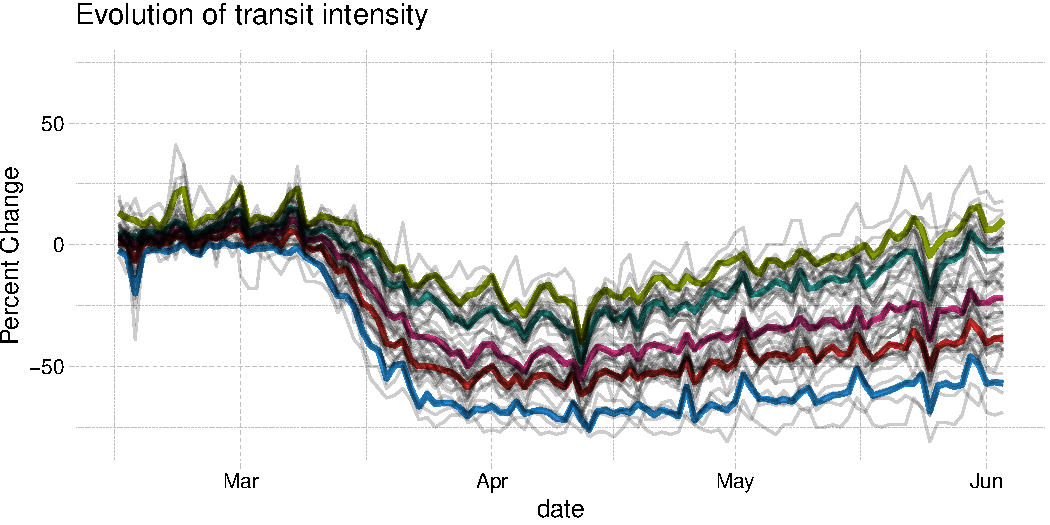
\includegraphics[width=0.6\linewidth]{../tables_and_figures/transit}\\
      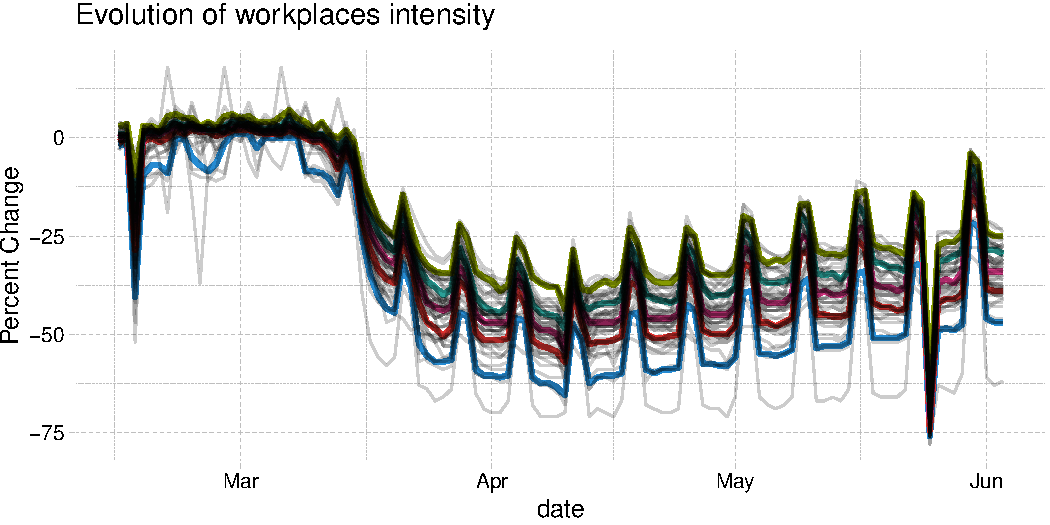
\includegraphics[width=0.6\linewidth]{../tables_and_figures/workplaces}
       \end{tabular}
        \begin{flushleft}
%        \scriptsize{This figure shows the evolution of ``Transit stations'' and  ``Workplaces'' of Google Mobility
%      Reports. Thin gray lines are the value in each state and date. Thicker colored lines are
%      quantiles of the variables conditional on date.}
      \end{flushleft}
\end{figure}

<<<<<<< HEAD
  
\end{frame}
%----------------------------------------------------------------------------------------%
 
=======

\end{frame}
%----------------------------------------------------------------------------------------%

>>>>>>> counterfactuals


%%----------------------------------------------------------------------------------------%
%
%\begin{frame}
%  \frametitle{Correlations between policy variables and behavior variables}\vspace{-0.05cm}
%  \begin{table}%\caption{Correlations among Policies and Behavior \label{tab:correlation}}\vspace{-0.2cm}
%  \begin{minipage}{\linewidth}
%    \resizebox{\linewidth}{!}{
%      
\begin{tabular}{lccccccccccc}
\toprule
\rotatebox{90}{ } & \rotatebox{90}{workplaces} & \rotatebox{90}{retail} & \rotatebox{90}{grocery} & \rotatebox{90}{transit} & \rotatebox{90}{masks for employees} & \rotatebox{90}{closed K-12 schools} & \rotatebox{90}{stay at home} & \rotatebox{90}{closed movie theaters} & \rotatebox{90}{closed restaurants} & \rotatebox{90}{closed non-essent bus} & \rotatebox{90}{business closure policies}\\
\midrule
workplaces & 1.00 &  &  &  &  &  &  &  &  &  & \\
retail & 0.93 & 1.00 &  &  &  &  &  &  &  &  & \\
grocery & 0.75 & 0.83 & 1.00 &  &  &  &  &  &  &  & \\
transit & 0.89 & 0.92 & 0.83 & 1.00 &  &  &  &  &  &  & \\
masks for employees & -0.32 & -0.17 & -0.15 & -0.29 & 1.00 &  &  &  &  &  & \\
\addlinespace
closed K-12 schools & -0.91 & -0.79 & -0.55 & -0.72 & 0.43 & 1.00 &  &  &  &  & \\
stay at home & -0.69 & -0.69 & -0.70 & -0.71 & 0.28 & 0.62 & 1.00 &  &  &  & \\
closed movie theaters & -0.81 & -0.76 & -0.64 & -0.71 & 0.34 & 0.82 & 0.72 & 1.00 &  &  & \\
closed restaurants & -0.77 & -0.82 & -0.68 & -0.76 & 0.21 & 0.74 & 0.72 & 0.82 & 1.00 &  & \\
closed non-essent bus & -0.65 & -0.68 & -0.68 & -0.64 & 0.08 & 0.56 & 0.76 & 0.68 & 0.71 & 1.00 & \\
\addlinespace
business closure policies & -0.84 & -0.84 & -0.75 & -0.79 & 0.24 & 0.78 & 0.81 & 0.92 & 0.93 & 0.87 & 1.00\\
\bottomrule
\end{tabular}
%    }\smallskip
%       \begin{flushleft}
%         \scriptsize
%         Each off-diagonal entry reports a correlation coefficient of
%         a pair of policy and behavior variables.
%       \end{flushleft}
%  \end{minipage}
%\end{table}
<<<<<<< HEAD
%   
=======
%
>>>>>>> counterfactuals
%\end{frame}
%%----------------------------------------------------------------------------------------%

%----------------------------------------------------------------------------------------%

\begin{frame}
  \frametitle{Portion of states with each
    policy}\vspace{-0.05cm}

\begin{figure}[ht]%\caption{Portion of states with each   policy \label{fig:policyportion}}
  \begin{minipage}{\linewidth}
    \begin{tabular}{ccc}
      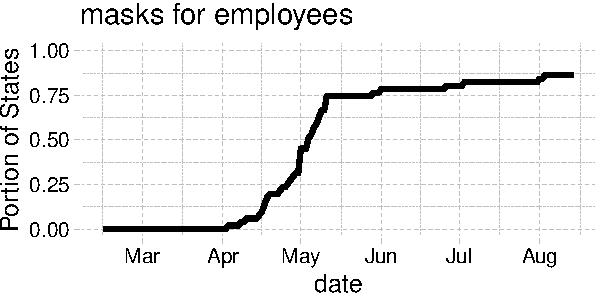
\includegraphics[width=0.33\textwidth]{../tables_and_figures/pmaskbus_p}
      &
        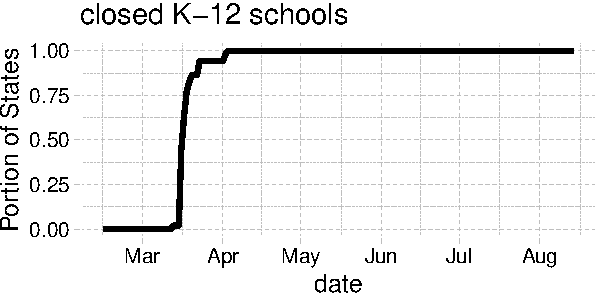
\includegraphics[width=0.33\textwidth]{../tables_and_figures/pk12_p}
      &
        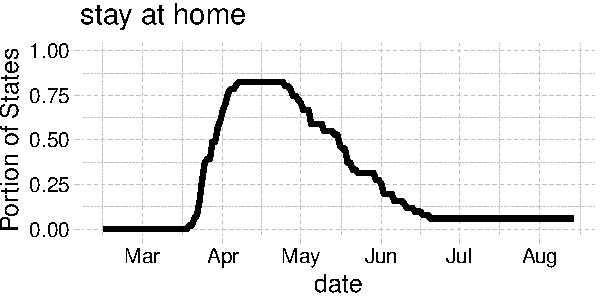
\includegraphics[width=0.33\textwidth]{../tables_and_figures/pshelter_p}
      \\
      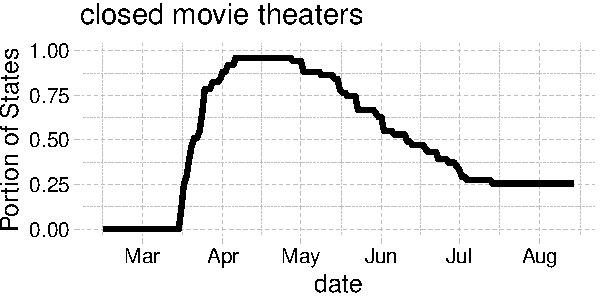
\includegraphics[width=0.33\textwidth]{../tables_and_figures/pmovie_p}
      &
        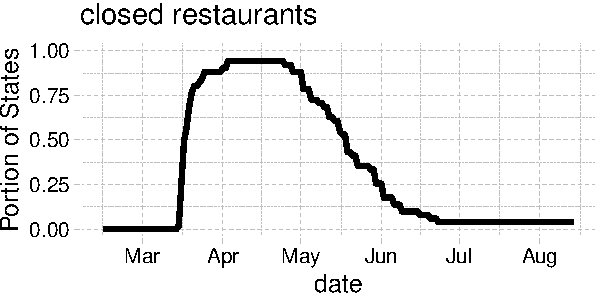
\includegraphics[width=0.33\textwidth]{../tables_and_figures/prestaurant_p}
      &
        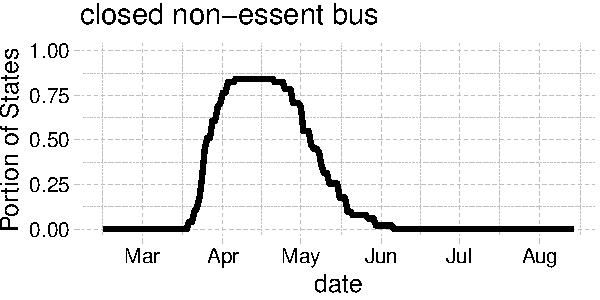
\includegraphics[width=0.33\textwidth]{../tables_and_figures/pnonessential_p}
    \end{tabular}
  \end{minipage}
\end{figure}


<<<<<<< HEAD
   
=======

\end{frame}
%----------------------------------------------------------------------------------------%



%----------------------------------------------------------------------------------------%

\begin{frame}
  \frametitle{Case and death growth conditional on mask mandates }\vspace{-0.05cm}



\begin{figure}[ht]
  %\caption{Case and death growth conditional on mask mandates \label{fig:masks}}\vspace{0.2cm}
  \begin{minipage}{\linewidth}
    \centering
    \begin{tabular}{cc}
      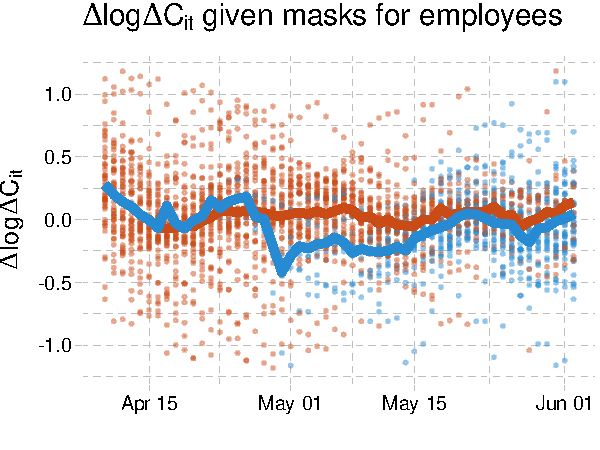
\includegraphics[width=0.483\textwidth]{../tables_and_figures/pmaskbus-cases}
      &
        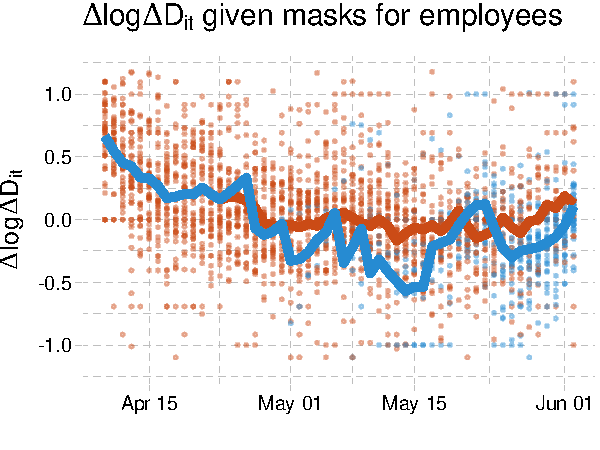
\includegraphics[width=0.483\textwidth]{../tables_and_figures/pmaskbus-deaths}
    \end{tabular}
%    \begin{flushleft}
%      \scriptsize In these figures, red points are the case or death
%      growth rate in states without a mask mandate. Blue points are
%      states with a mask mandate 14 (21 for deaths) days prior. The
%      red line is the average across states without a mask mandate 14
%      (21 for deaths) days earlier. The blue line is the average
%      across states with a mask mandate 14 (21 for deaths) earlier.
%    \end{flushleft}
  \end{minipage}
\end{figure}


\end{frame}
%----------------------------------------------------------------------------------------%



%----------------------------------------------------------------------------------------%

\begin{frame}
  \frametitle{Regression Analysis}

% We first examine how policies and information affect social distancing behaviors by estimating a version of (\ref{eq:R2}):
	\begin{align}
   &  {\ycolor  Y_{it}}
    = {\bcolor\alpha ' B_{it}} + {\pcolor\pi 'P_{it}} + {\icolor\mu'I_{it}} + {\wcolor\delta_Y 'W_{it}}  + \varepsilon^y_{it} \tag{BPI$\to$Y}\\
   % &  & \varepsilon^y_{it} \perp {\bcolor B_{it}}, {\pcolor P_{it}}, {\icolor I_{it}}, {\wcolor W_{it}} \label{eq:R1} \tag{BPI$\to$Y} \\
    &  {\bcolor B_{it}^j}
     =  {\pcolor \beta' P_{it}} + {\icolor \gamma'I_{it}} +  {\wcolor \delta_B' W_{it}} + \varepsilon^b_{it} \tag{PI$\to$B}\\
   \notag  \\
  % & & \varepsilon^b_{it} \perp {\pcolor P_{it}}, {\icolor I_{it}}, {\wcolor W_{it}}  \label{eq:R2} \tag{PI$\to$B} % \\
%    & {\pcolor P_{it}}
%    =  {\icolor\eta'I_{it}} + {\wcolor \delta_P' W_{it}} +   \varepsilon^p_{it},   & & \varepsilon^p_{it} \perp   {\icolor I_{it}}, {\wcolor W_{it}} \label{eq:R3}  \tag{I$\to$P}
 &  {\ycolor  Y_{it}}
   = ( {\pcolor\pi'}+ {\bcolor\alpha '}  {\pcolor \beta' }  )
    {\pcolor P_{it}} + (  {\icolor  \mu'}+{\bcolor\alpha '}  {\icolor \gamma'})
    {\icolor I_{it} }+ {\wcolor \bar \delta 'W_{it}}  + \bar \varepsilon_{it}. \tag{PI$\to$Y}
       \end{align}

\begin{itemize}
\item ${\ycolor Y_{it}}$:  the growth rate of cases or deaths\smallskip
\item   ${\bcolor B_{it}^j}$:  ``Transit,''  ``Workplaces''  ``Grocery," and ``Retail''  lagged by 14 or 21 days\smallskip
\item  $ {\pcolor  P_{it}} $:  various policies  lagged by 14 or 21 days\smallskip
\item $ {\icolor I_{it}} $: past cases/deaths,  national-level cases/deaths etc.\smallskip
\item $ {\wcolor   W_{it}}$: state-level characteristics   and month dummies.
\end{itemize}


\end{frame}
%----------------------------------------------------------------------------------------%


%----------------------------------------------------------------------------------------%

\begin{frame}
  \frametitle{Direct and Indirect Policy Effects for Case Regression}

\begin{table}
 % \caption{\label{tab:dieff}Direct and Indirect Policy Effects}
\begin{minipage}{\linewidth}
  \centering
    \tiny
  \begin{tabular}{c}
%    \textbf{Cases}
%    \\
%    \input{tables_and_figures/dieff-cases}
      \\
    \textbf{{\normalsize Case Growth Regression}}
    \\
    \\
\begin{tabular}{lccc|c|cc}
\toprule
&\multicolumn{3}{c|}{ PI$\to$B Coef.\ \& \ PBI$\to$Y Coef.  } &PI$\to$Y Coef.  \\
  & Direct & Indirect & Total & Total  & Difference & Average\\\
  &${\pcolor\pi'}$&${\bcolor\alpha '}  {\pcolor \beta' }$ &${\pcolor\pi'}+{\bcolor\alpha '}  {\pcolor \beta' }$ &${\pcolor\pi'}+{\bcolor\alpha '}  {\pcolor \beta' }$ & (over-id test)  \\
\midrule
masks for employees & -0.097$^{***}$ & -0.019 & -0.116$^{***}$ & -0.105$^{***}$ & -0.011 & -0.111$^{***}$\\
 & (0.032) & (0.015) & (0.038) & (0.037) & (0.010) & (0.037)\\
closed K-12 schools & 0.025 & -0.021 & 0.004 & 0.009 & -0.005 & 0.007\\
 & (0.101) & (0.038) & (0.110) & (0.108) & (0.016) & (0.109)\\
stay at home & -0.064 & -0.047$^{**}$ & -0.112$^{**}$ & -0.117$^{**}$ & 0.005 & -0.114$^{**}$\\
 & (0.047) & (0.021) & (0.051) & (0.052) & (0.009) & (0.051)\\
closed movie theaters & 0.053 & -0.002 & 0.051 & 0.058 & -0.006 & 0.055\\
 & (0.048) & (0.017) & (0.050) & (0.048) & (0.010) & (0.048)\\
closed restaurants & 0.021 & -0.038$^{**}$ & -0.017 & -0.010 & -0.008 & -0.013\\
 & (0.047) & (0.019) & (0.044) & (0.046) & (0.011) & (0.045)\\
closed businesses & -0.016 & -0.013 & -0.028 & -0.035 & 0.006 & -0.032\\
 & (0.042) & (0.012) & (0.045) & (0.045) & (0.008) & (0.045)\\
 \midrule
$\sum_j \mathrm{Policy}_j$ & -0.078 & -0.140$^{**}$ & -0.218 & -0.199 & -0.019 & -0.209\\
 & (0.158) & (0.059) & (0.165) & (0.164) & (0.018) & (0.164)\\
%$\Delta \log \Delta C_{it}$ & 0.023 & 0.010 & 0.033 & 0.033 & -0.000 & 0.033\\
%\addlinespace
% & (0.028) & (0.007) & (0.028) & (0.028) & (0.003) & (0.028)\\
%$\log \Delta C_{it}$ & -0.089$^{***}$ & 0.001 & -0.088$^{***}$ & -0.091$^{***}$ & 0.003 & -0.090$^{***}$\\
% & (0.021) & (0.010) & (0.027) & (0.026) & (0.004) & (0.026)\\
%$\Delta \log \Delta C_{it}$.national & -0.090$^{**}$ & -0.040$^{***}$ & -0.130$^{***}$ & -0.123$^{***}$ & -0.006 & -0.126$^{***}$\\
% & (0.043) & (0.016) & (0.043) & (0.042) & (0.013) & (0.042)\\
%\addlinespace
%$\log \Delta C_{it}$.national & -0.184$^{***}$ & -0.068$^{***}$ & -0.252$^{***}$ & -0.241$^{***}$ & -0.010 & -0.247$^{***}$\\
% & (0.049) & (0.023) & (0.045) & (0.045) & (0.010) & (0.045)\\
\bottomrule
\end{tabular}

    \\
  \end{tabular}
%  \smallskip
%  \begin{flushleft}
%      \scriptsize Direct effects capture the effect of policy on case
%      growth holding behavior, information, and confounders
%      constant. Direct effects are given by ${\pcolor \pi}$ in
%      equation (\ref{eq:R1}). Indirect effects capture how policy
%      changes behavior and behavior shift case growth. They are given
%      by ${\bcolor \alpha}$ from (\ref{eq:R1}) times ${\pcolor \beta}$
%      from (\ref{eq:R2}). The total effect is
%      ${\pcolor \pi} + {\pcolor \beta} {\bcolor \alpha}$. Column
%      ``PI$\to$Y Coefficients'' shows the coefficient estimates from
%      \ref{eq:R4}. Columns ``Difference''    are  the differences between
%      the estimates from (\ref{eq:R4}) and the combination of
%      (\ref{eq:R1}) and (\ref{eq:R2}) while column ``Average'' are their averages.
%      Standard errors are computed by
%      bootstrap and clustered on state.
%    %  \ref{tab:PtoY}.
%    \end{flushleft}
  \end{minipage}
\end{table}
\end{frame}
%----------------------------------------------------------------------------------------%


%----------------------------------------------------------------------------------------%

\begin{frame}
  \frametitle{Direct and Indirect Policy Effects for Death Regression}

\begin{table}
 % \caption{\label{tab:dieff}Direct and Indirect Policy Effects}
\begin{minipage}{\linewidth}
  \centering
    \tiny
  \begin{tabular}{c}
%    \textbf{Cases}
%    \\
%    \input{tables_and_figures/dieff-cases}
      \\
    \textbf{{\normalsize Death Growth Regression}}
    \\
    \\
\begin{tabular}{lccc|c|cc}
\toprule
&\multicolumn{3}{c|}{ PI$\to$B Coef.\ \& \ PBI$\to$Y Coef.  } &PI$\to$Y Coef.  \\
  & Direct & Indirect & Total & Total  & Difference & Average\\\
  &${\pcolor\pi'}$&${\bcolor\alpha '}  {\pcolor \beta' }$ &${\pcolor\pi'}+{\bcolor\alpha '}  {\pcolor \beta' }$ &${\pcolor\pi'}+{\bcolor\alpha '}  {\pcolor \beta' }$  & (over-id test) \\
\midrule
masks for employees & -0.148$^{***}$ & -0.018 & -0.166$^{***}$ & -0.161$^{***}$ & -0.005 & -0.164$^{***}$\\
 & (0.049) & (0.022) & (0.054) & (0.051) & (0.015) & (0.052)\\
closed K-12 schools & -0.199$^{**}$ & -0.038 & -0.238$^{**}$ & -0.250$^{**}$ & 0.012 & -0.244$^{**}$\\
 & (0.092) & (0.039) & (0.104) & (0.102) & (0.020) & (0.103)\\
stay at home & -0.047 & -0.030 & -0.077 & -0.075 & -0.002 & -0.076\\
%\addlinespace
 & (0.062) & (0.033) & (0.061) & (0.061) & (0.013) & (0.061)\\
closed movie theaters & 0.054 & 0.007 & 0.061 & 0.065 & -0.004 & 0.063\\
 & (0.087) & (0.021) & (0.083) & (0.081) & (0.015) & (0.082)\\
closed restaurants & 0.081 & -0.058$^{**}$ & 0.023 & 0.031 & -0.008 & 0.027\\
 & (0.065) & (0.025) & (0.053) & (0.053) & (0.014) & (0.052)\\
%\addlinespace
closed businesses & -0.003 & 0.003 & -0.000 & -0.012 & 0.012 & -0.006\\
 & (0.057) & (0.016) & (0.060) & (0.062) & (0.011) & (0.060)\\ \midrule
$\sum_j \mathrm{Policy}_j$ & -0.262 & -0.135 & -0.397$^{**}$ & -0.402$^{**}$ & 0.005 & -0.399$^{**}$\\
 & (0.172) & (0.088) & (0.180) & (0.176) & (0.022) & (0.178)\\
%$\Delta \log \Delta D_{it}$ & 0.017 & -0.002 & 0.015 & 0.019 & -0.004 & 0.017\\
%\addlinespace
% & (0.036) & (0.005) & (0.035) & (0.036) & (0.004) & (0.035)\\
%$\log \Delta D_{it}$ & -0.049$^{**}$ & -0.006 & -0.055$^{**}$ & -0.062$^{**}$ & 0.007 & -0.059$^{**}$\\
% & (0.024) & (0.009) & (0.027) & (0.027) & (0.005) & (0.027)\\
%$\Delta \log \Delta D_{it}$.national & -0.046 & -0.069$^{***}$ & -0.115$^{**}$ & -0.160$^{***}$ & 0.045$^{***}$ & -0.137$^{***}$\\
% & (0.044) & (0.021) & (0.049) & (0.056) & (0.013) & (0.052)\\
%\addlinespace
%$\log \Delta D_{it}$.national & -0.060 & -0.097$^{***}$ & -0.157$^{***}$ & -0.120$^{***}$ & -0.037$^{***}$ & -0.138$^{***}$\\
% & (0.037) & (0.028) & (0.034) & (0.030) & (0.012) & (0.032)\\
\bottomrule
\end{tabular}
    \\
  \end{tabular}
%  \smallskip
%  \begin{flushleft}
%      \scriptsize Direct effects capture the effect of policy on case
%      growth holding behavior, information, and confounders
%      constant. Direct effects are given by ${\pcolor \pi}$ in
%      equation (\ref{eq:R1}). Indirect effects capture how policy
%      changes behavior and behavior shift case growth. They are given
%      by ${\bcolor \alpha}$ from (\ref{eq:R1}) times ${\pcolor \beta}$
%      from (\ref{eq:R2}). The total effect is
%      ${\pcolor \pi} + {\pcolor \beta} {\bcolor \alpha}$. Column
%      ``PI$\to$Y Coefficients'' shows the coefficient estimates from
%      \ref{eq:R4}. Columns ``Difference''    are  the differences between
%      the estimates from (\ref{eq:R4}) and the combination of
%      (\ref{eq:R1}) and (\ref{eq:R2}) while column ``Average'' are their averages.
%      Standard errors are computed by
%      bootstrap and clustered on state.
%    %  \ref{tab:PtoY}.
%    \end{flushleft}
  \end{minipage}
\end{table}
\end{frame}
%----------------------------------------------------------------------------------------%


%----------------------------------------------------------------------------------------%

\begin{frame}
  \frametitle{The Effect of Policies and Information on Behavior (PI$\to$ B)}

  % \textbf{Plan: will only present (5)-(8) columns}
  % behavior-deathsinfo-nationinfo-pib is columns (5)-(8)
  % behavior-deathsinfo-stateinfo-pib is columns (1)-(4)
  % for cases:
  % behavior-cases-nationinfo-pib is columns (5)-(8)
  % behavior-cases-stateinfo-pib is columns (1)-(4)

\begin{table}
      \begin{minipage}{\linewidth}
        \centering
        \resizebox*{!}{\dimexpr\textheight-2\baselineskip\relax}{
            \begin{tabular}{@{\extracolsep{1pt}}lcccc} 
\\[-1.8ex]\hline 
\hline \\[-1.8ex] 
 & \multicolumn{4}{c}{\textit{Dependent variable:}} \\ 
\cline{2-5} 
 & workplaces & retail & grocery & transit \\ 
\\[-1.8ex] & (1) & (2) & (3) & (4)\\ 
\hline \\[-1.8ex] 
 masks for employees & 0.001 & 0.005 & 0.008 & $-$0.017 \\ 
  & (0.010) & (0.017) & (0.012) & (0.026) \\ 
  closed K-12 schools & $-$0.044$^{***}$ & $-$0.037$^{**}$ & $-$0.025 & $-$0.049 \\ 
  & (0.015) & (0.018) & (0.021) & (0.039) \\ 
  stay at home & $-$0.025$^{**}$ & $-$0.034$^{**}$ & $-$0.071$^{***}$ & $-$0.069$^{**}$ \\ 
  & (0.012) & (0.015) & (0.018) & (0.032) \\ 
  business closure policies & $-$0.044$^{***}$ & $-$0.095$^{***}$ & $-$0.069$^{***}$ & $-$0.052 \\ 
  & (0.012) & (0.022) & (0.021) & (0.039) \\ 
  $\Delta \log \Delta D_{it}$ & 0.001 & $-$0.008$^{*}$ & $-$0.006 & $-$0.004 \\ 
  & (0.002) & (0.005) & (0.005) & (0.005) \\ 
  $\log \Delta D_{it}$ & $-$0.008$^{*}$ & 0.0003 & 0.004 & $-$0.003 \\ 
  & (0.004) & (0.007) & (0.006) & (0.011) \\ 
  $\Delta \log \Delta D_{it}$.national & $-$0.057$^{***}$ & $-$0.093$^{***}$ & $-$0.014$^{***}$ & $-$0.067$^{***}$ \\ 
  & (0.004) & (0.007) & (0.005) & (0.009) \\ 
  $\log \Delta D_{it}$.national & $-$0.054$^{***}$ & $-$0.059$^{***}$ & $-$0.034$^{***}$ & $-$0.053$^{***}$ \\ 
  & (0.004) & (0.007) & (0.006) & (0.011) \\ 
 \hline \\[-1.8ex] 
state variables & Yes & Yes & Yes & Yes \\ 
Month $\times$ state variables & Yes & Yes & Yes & Yes \\ 
\hline \\[-1.8ex] 
$\sum_j \mathrm{Policy}_j$ & -0.112$^{***}$ & -0.161$^{***}$ & -0.158$^{***}$ & -0.186$^{***}$ \\ 
 & (0.024) & (0.039) & (0.036) & (0.068) \\ 
Observations & 3,468 & 3,468 & 3,468 & 3,468 \\ 
R$^{2}$ & 0.956 & 0.906 & 0.790 & 0.862 \\ 
Adjusted R$^{2}$ & 0.956 & 0.905 & 0.788 & 0.861 \\ 
\hline 
\hline \\[-1.8ex] 
\textit{Note:}  & \multicolumn{4}{r}{$^{*}$p$<$0.1; $^{**}$p$<$0.05; $^{***}$p$<$0.01} \\ 
\end{tabular} 
          }
        \begin{flushleft}
          \scriptsize
%          Dependent variables are   ``Transit
%          Intensity,'' ``Workplace Intensity,'' ``Retail Intensity,'' and ``Grocery
%          Intensity" defined as 7 days moving averages of corresponding daily measures obtained from Google Mobility Reports.  All specifications include state-level characteristics (population, area, unemployment rate, poverty rate, and a percentage of people subject to illness) as well as their interactions with the log of days since Jan 15, 2020. The row ``$\sum_j \text{Policy}_j$'' reports the sum of six policy coefficients.
        \end{flushleft}
      \end{minipage}
      \end{table}

\end{frame}
%----------------------------------------------------------------------------------------%




%%----------------------------------------------------------------------------------------%
%
%\begin{frame}
%  \frametitle{The Effect of Policies, Behavior, and Information on Case/Death Growth}
%
%Case Growth Regression:
%\begin{align}
% {\ycolor   \Delta \log \Delta C_{it}}
%    = {\bcolor\alpha ' B_{it}} + {\pcolor\pi 'P_{it}} + {\icolor\mu'I_{it}} + {\wcolor\delta_Y 'W_{it}}  + \varepsilon^y_{it},
% %   &  & \varepsilon^y_{it} \perp {\bcolor B_{it}}, {\pcolor P_{it}}, {\icolor I_{it}}, {\wcolor W_{it}}
%     \notag
%\end{align}
%
%Death Growth Regression:
%\begin{align}
% {\ycolor   \Delta \log \Delta D_{it}}
%    = {\bcolor\alpha ' B_{it}} + {\pcolor\pi 'P_{it}} + {\icolor\mu'I_{it}} + {\wcolor\delta_Y 'W_{it}}  + \varepsilon^y_{it},
% %   &  & \varepsilon^y_{it} \perp {\bcolor B_{it}}, {\pcolor P_{it}}, {\icolor I_{it}}, {\wcolor W_{it}}
%     \notag
%\end{align}
%
%%\begin{itemize}
%%\item ${\ycolor Y_{it}}= \Delta \log \Delta C_{it}$ or  $\Delta \log \Delta D_{it}$
%%%\item   ${\bcolor B_{it}^j}$:  ``Transit,''  ``Workplaces''  ``Grocery," and ``Retail'' \smallskip
%%%\item  $ {\pcolor  P_{it}} $ various policies \smallskip
%%%\item $ {\icolor I_{it}} $: past  cases/deaths etc. \smallskip
%%%\item $ {\wcolor   W_{it}}$: state-level characteristics   and month dummies.
%%\end{itemize}
%
%
%\end{frame}
%%----------------------------------------------------------------------------------------%



%----------------------------------------------------------------------------------------%

\begin{frame}
  \frametitle{The Direct Effect of Policies, Behavior, and Information on Case/Death Growth (BPI$\to$Y)}

%\textbf{Plan: will only present (1) and (3) columns for each table, possibly only for death growth}


\begin{table}[!htbp] \centering
% \caption{The Direct Effect of Behavior and Policies on Case and
%   Death Growth ($PBI \to Y$)}\vspace{-0.3cm}
 \label{tab:BPItoY}
 \begin{minipage}{\linewidth}
   \centering
   \resizebox*{!}{\dimexpr\textheight-2\baselineskip\relax}{
     \scriptsize
   \begin{tabular}{cc}
   \begin{minipage}{\linewidth}
     \centering
     \begin{tabular}{@{\extracolsep{1pt}}lcc} 
\\[-1.8ex]\hline 
\hline \\[-1.8ex] 
 & \multicolumn{2}{c}{\textit{Dependent variable:}} \\ 
\cline{2-3} 
 & \multicolumn{2}{c}{$\Delta \log \Delta C_{it}$} \\ 
\\[-1.8ex] & (1) & (2)\\ 
\hline \\[-1.8ex] 
 lag(masks for employees, 14) & $-$0.090$^{***}$ & $-$0.100$^{***}$ \\ 
  & (0.031) & (0.029) \\ 
  lag(closed K-12 schools, 14) & $-$0.074 & 0.043 \\ 
  & (0.080) & (0.096) \\ 
  lag(stay at home, 14) & $-$0.063 & $-$0.079 \\ 
  & (0.050) & (0.052) \\ 
  lag(business closure policies, 14) & 0.051 & 0.045 \\ 
  & (0.062) & (0.060) \\ 
  lag(workplaces, 14) & 1.055$^{*}$ & 0.391 \\ 
  & (0.543) & (0.610) \\ 
  lag(retail, 14) & 0.594$^{*}$ & 0.316 \\ 
  & (0.303) & (0.316) \\ 
  lag(grocery, 14) & $-$0.471$^{*}$ & $-$0.259 \\ 
  & (0.284) & (0.282) \\ 
  lag(transit, 14) & 0.347 & 0.355 \\ 
  & (0.258) & (0.247) \\ 
  lag($\Delta \log \Delta C_{it}$, 14) & 0.015 & 0.024 \\ 
  & (0.026) & (0.028) \\ 
  lag($\log \Delta C_{it}$, 14) & $-$0.105$^{***}$ & $-$0.088$^{***}$ \\ 
  & (0.019) & (0.021) \\ 
  lag($\Delta \log \Delta C_{it}$.national, 14) &  & $-$0.095$^{**}$ \\ 
  &  & (0.042) \\ 
  lag($\log \Delta C_{it}$.national, 14) &  & $-$0.177$^{***}$ \\ 
  &  & (0.049) \\ 
  $\Delta \log T_{it}$ & 0.152$^{***}$ & 0.155$^{***}$ \\ 
  & (0.043) & (0.042) \\ 
 \hline \\[-1.8ex] 
state variables & Yes & Yes \\ 
Month $\times$ state variables & Yes & Yes \\ 
\hline \\[-1.8ex] 
$\sum_j \mathrm{Policy}_j$ & -0.176 & -0.091 \\ 
 & (0.128) & (0.153) \\ 
$\sum_k w_k \mathrm{Behavior}_k$ & -0.804$^{***}$ & -0.425$^{***}$ \\ 
 & (0.140) & (0.157) \\ 
Observations & 3,825 & 3,825 \\ 
R$^{2}$ & 0.761 & 0.766 \\ 
Adjusted R$^{2}$ & 0.759 & 0.763 \\ 
\hline 
\hline \\[-1.8ex] 
\textit{Note:}  & \multicolumn{2}{r}{$^{*}$p$<$0.1; $^{**}$p$<$0.05; $^{***}$p$<$0.01} \\ 
\end{tabular} 
   \end{minipage}
     %\hspace{1pt}
     &
   \begin{minipage}{\linewidth}
     \centering
     \begin{tabular}{@{\extracolsep{1pt}}lcc} 
\\[-1.8ex]\hline 
\hline \\[-1.8ex] 
 & \multicolumn{2}{c}{\textit{Dependent variable:}} \\ 
\cline{2-3} 
 & \multicolumn{2}{c}{$\Delta \log \Delta D_{it}$} \\ 
\\[-1.8ex] & (1) & (2)\\ 
\hline \\[-1.8ex] 
 lag(masks for employees, 21) & $-$0.146$^{***}$ & $-$0.147$^{***}$ \\ 
  & (0.050) & (0.049) \\ 
  lag(closed K-12 schools, 21) & $-$0.232$^{**}$ & $-$0.178$^{*}$ \\ 
  & (0.102) & (0.103) \\ 
  lag(stay at home, 21) & $-$0.066 & $-$0.065 \\ 
  & (0.067) & (0.067) \\ 
  lag(business closure policies, 21) & 0.098 & 0.107 \\ 
  & (0.087) & (0.092) \\ 
  lag(workplaces, 21) & 1.297$^{**}$ & 0.896 \\ 
  & (0.515) & (0.554) \\ 
  lag(retail, 21) & 0.572 & 0.523 \\ 
  & (0.441) & (0.438) \\ 
  lag(grocery, 21) & $-$0.935$^{**}$ & $-$0.887$^{**}$ \\ 
  & (0.388) & (0.368) \\ 
  lag(transit, 21) & 0.348 & 0.384 \\ 
  & (0.284) & (0.283) \\ 
  lag($\Delta \log \Delta D_{it}$, 21) & 0.016 & 0.016 \\ 
  & (0.035) & (0.037) \\ 
  lag($\log \Delta D_{it}$, 21) & $-$0.055$^{**}$ & $-$0.053$^{**}$ \\ 
  & (0.024) & (0.024) \\ 
  lag($\Delta \log \Delta D_{it}$.national, 21) &  & $-$0.034 \\ 
  &  & (0.044) \\ 
  lag($\log \Delta D_{it}$.national, 21) &  & $-$0.047 \\ 
  &  & (0.039) \\ 
   &  &  \\ 
  &  &  \\ 
 \hline \\[-1.8ex] 
state variables & Yes & Yes \\ 
Month $\times$ state variables & Yes & Yes \\ 
\hline \\[-1.8ex] 
$\sum_j \mathrm{Policy}_j$ & -0.346$^{**}$ & -0.283$^{*}$ \\ 
 & (0.162) & (0.172) \\ 
$\sum_k w_k \mathrm{Behavior}_k$ & -0.837$^{***}$ & -0.661$^{***}$ \\ 
 & (0.164) & (0.176) \\ 
Observations & 3,468 & 3,468 \\ 
R$^{2}$ & 0.518 & 0.518 \\ 
Adjusted R$^{2}$ & 0.512 & 0.513 \\ 
\hline 
\hline \\[-1.8ex] 
\textit{Note:}  & \multicolumn{2}{r}{$^{*}$p$<$0.1; $^{**}$p$<$0.05; $^{***}$p$<$0.01} \\ 
\end{tabular} 
   \end{minipage}
   \end{tabular}
   }
% \begin{flushleft}
%     \scriptsize Dependent variable is the weekly growth rate of
%     confirmed cases (in the left panel) or deaths (in the right
%     panel) as defined in equation (\ref{eq:y}). The covariates
%     include lagged policy and behavior variables, which are
%     constructed as 7 day moving averages between $t$ to $t-7$ of
%     corresponding daily measures.  The row
%     ``$\sum_j \mathrm{Policies}_j$'' reports the sum of six policy
%     coefficients.  The row ``$\sum_k w_k \mathrm{Behavior}_k$''
%     reports the sum of four coefficients of behavior variables
%     weighted by the average of each behavioral variable from April
%     1st-10th.
%   \end{flushleft}
 \end{minipage}
\end{table}

\end{frame}
%----------------------------------------------------------------------------------------%



%----------------------------------------------------------------------------------------%

\begin{frame}
  \frametitle{The Total Effect of Policies and Information on Case/Death Growth (PI$\to$ Y)}

%\textbf{Plan: will only present (1) and (3) columns for each table, possibly only for death growth}

\begin{table}[!htbp] \centering
% \caption{\label{tab:PtoY}
%   The Total Effect of Policies on Case and Death Growth ($PI \to Y$)}\vspace{-0.3cm}
 \begin{minipage}{\linewidth}
   \centering
   \resizebox*{!}{\dimexpr\textheight-2\baselineskip\relax}{
        %\resizebox{\textwidth}{!}{
   \centering
   \footnotesize
   \begin{tabular}{cc}
   \begin{minipage}{\linewidth}
     \centering
     \begin{tabular}{@{\extracolsep{1pt}}lcc} 
\\[-1.8ex]\hline 
\hline \\[-1.8ex] 
 & \multicolumn{2}{c}{\textit{Dependent variable:}} \\ 
\cline{2-3} 
 & \multicolumn{2}{c}{$\Delta \log \Delta C_{it}$} \\ 
\\[-1.8ex] & (1) & (2)\\ 
\hline \\[-1.8ex] 
 lag(masks for employees, 14) & $-$0.083$^{**}$ & $-$0.103$^{***}$ \\ 
  & (0.038) & (0.033) \\ 
  lag(closed K-12 schools, 14) & $-$0.226$^{**}$ & 0.029 \\ 
  & (0.089) & (0.102) \\ 
  lag(stay at home, 14) & $-$0.127$^{**}$ & $-$0.115$^{**}$ \\ 
  & (0.057) & (0.054) \\ 
  lag(business closure policies, 14) & $-$0.076 & $-$0.001 \\ 
  & (0.068) & (0.061) \\ 
  lag($\Delta \log \Delta C_{it}$, 14) & 0.040 & 0.036 \\ 
  & (0.024) & (0.028) \\ 
  lag($\log \Delta C_{it}$, 14) & $-$0.137$^{***}$ & $-$0.091$^{***}$ \\ 
  & (0.022) & (0.026) \\ 
  lag($\Delta \log \Delta C_{it}$.national, 14) &  & $-$0.128$^{***}$ \\ 
  &  & (0.039) \\ 
  lag($\log \Delta C_{it}$.national, 14) &  & $-$0.243$^{***}$ \\ 
  &  & (0.045) \\ 
  $\Delta \log T_{it}$ & 0.156$^{***}$ & 0.158$^{***}$ \\ 
  & (0.044) & (0.042) \\ 
 \hline \\[-1.8ex] 
state variables & Yes & Yes \\ 
Month $\times$ state variables & Yes & Yes \\ 
\hline \\[-1.8ex] 
$\sum_j \mathrm{Policy}_j$ & -0.512$^{***}$ & -0.190 \\ 
 & (0.150) & (0.156) \\ 
Observations & 3,825 & 3,825 \\ 
R$^{2}$ & 0.749 & 0.763 \\ 
Adjusted R$^{2}$ & 0.747 & 0.760 \\ 
\hline 
\hline \\[-1.8ex] 
\textit{Note:}  & \multicolumn{2}{r}{$^{*}$p$<$0.1; $^{**}$p$<$0.05; $^{***}$p$<$0.01} \\ 
\end{tabular} 
   \end{minipage}
     &
   \begin{minipage}{\linewidth}
     \centering
     \begin{tabular}{@{\extracolsep{1pt}}lcc} 
\\[-1.8ex]\hline 
\hline \\[-1.8ex] 
 & \multicolumn{2}{c}{\textit{Dependent variable:}} \\ 
\cline{2-3} 
 & \multicolumn{2}{c}{$\Delta \log \Delta D_{it}$} \\ 
\\[-1.8ex] & (1) & (2)\\ 
\hline \\[-1.8ex] 
 lag(masks for employees, 21) & $-$0.134$^{***}$ & $-$0.156$^{***}$ \\ 
  & (0.051) & (0.050) \\ 
  lag(closed K-12 schools, 21) & $-$0.610$^{***}$ & $-$0.234$^{**}$ \\ 
  & (0.115) & (0.111) \\ 
  lag(stay at home, 21) & $-$0.082 & $-$0.068 \\ 
  & (0.066) & (0.066) \\ 
  lag(business closure policies, 21) & $-$0.059 & 0.059 \\ 
  & (0.086) & (0.086) \\ 
  lag($\Delta \log \Delta D_{it}$, 21) & $-$0.001 & 0.017 \\ 
  & (0.033) & (0.036) \\ 
  lag($\log \Delta D_{it}$, 21) & $-$0.078$^{***}$ & $-$0.064$^{**}$ \\ 
  & (0.026) & (0.027) \\ 
  lag($\Delta \log \Delta D_{it}$.national, 21) &  & $-$0.147$^{***}$ \\ 
  &  & (0.056) \\ 
  lag($\log \Delta D_{it}$.national, 21) &  & $-$0.116$^{***}$ \\ 
  &  & (0.032) \\ 
   &  &  \\ 
  &  &  \\ 
 \hline \\[-1.8ex] 
state variables & Yes & Yes \\ 
Month $\times$ state variables & Yes & Yes \\ 
\hline \\[-1.8ex] 
$\sum_j \mathrm{Policy}_j$ & -0.885$^{***}$ & -0.399$^{**}$ \\ 
 & (0.159) & (0.183) \\ 
Observations & 3,468 & 3,468 \\ 
R$^{2}$ & 0.502 & 0.512 \\ 
Adjusted R$^{2}$ & 0.497 & 0.507 \\ 
\hline 
\hline \\[-1.8ex] 
\textit{Note:}  & \multicolumn{2}{r}{$^{*}$p$<$0.1; $^{**}$p$<$0.05; $^{***}$p$<$0.01} \\ 
\end{tabular} 
   \end{minipage}

   \end{tabular}
   }
%   \begin{flushleft}
%     \scriptsize Dependent variable is the weekly growth rate of
%     confirmed cases (in the left panel) or deaths (in the right
%     panel) as defined in equation (\ref{eq:y}). The covariates
%     include lagged policy variables, which are
%     constructed as 7 day moving averages between $t$ to $t-7$ of
%     corresponding daily measures.  The row
%     ``$\sum_j \mathrm{Policies}_j$'' reports the sum of six policy
%     coefficients.
%   \end{flushleft}
 \end{minipage}
\end{table}

\end{frame}
%----------------------------------------------------------------------------------------%


%----------------------------------------------------------------------------------------%

\begin{frame}
  \frametitle{Effect of mandating masks on April 1st in Washington }


\begin{figure}[ht]
%  \caption{Effect of mandating masks on April 1st in Washington \label{fig:WA-mask}}
  \begin{minipage}{\linewidth}
    \centering
    \begin{tabular}{cc}
      \includegraphics[width=0.45\textwidth]{../tables_and_figures/Washington-mask-growth}
      &
      \includegraphics[width=0.45\textwidth]{../tables_and_figures/Washington-mask-dgrowth}
    \end{tabular}
  \end{minipage}
\end{figure}
\begin{figure}[ht]
%  \caption{Effect of mandating masks on April 1st in Washington \label{fig:WA-mask}}
  \begin{minipage}{\linewidth}
    \centering
    \begin{tabular}{cc}
        \includegraphics[width=0.45\textwidth]{../tables_and_figures/Washington-mask-growth_deaths}
      &
        \includegraphics[width=0.45\textwidth]{../tables_and_figures/Washington-mask-dgrowth_deaths}
    \end{tabular}
  \end{minipage}
\end{figure}



\end{frame}
%----------------------------------------------------------------------------------------%


%----------------------------------------------------------------------------------------%

\begin{frame}
  \frametitle{Effect of mandating masks on April 1st: National average }

\begin{figure}[ht]
%  \caption{National change in cases from mandating masks on April
%    1st\label{fig:US-mask}}
  \begin{minipage}{\linewidth}
    \centering
    \begin{tabular}{cc}
      \includegraphics[width=0.45\textwidth]{../tables_and_figures/us-mask-dgrowth}
      &
        \includegraphics[width=0.45\textwidth]{../tables_and_figures/us-mask-rel}
    \end{tabular}
  \end{minipage}
\end{figure}

\begin{figure}[ht]
%  \caption{National change in deaths from mandating masks on April
%    1st\label{fig:US-mask-deaths}}
  \begin{minipage}{\linewidth}
    \centering
    \begin{tabular}{cc}
      \includegraphics[width=0.45\textwidth]{../tables_and_figures/us-mask-dgrowth_deaths}
      &
        \includegraphics[width=0.45\textwidth]{../tables_and_figures/us-mask-rel_deaths}
    \end{tabular}
  \end{minipage}
\end{figure}


\end{frame}
%----------------------------------------------------------------------------------------%






%----------------------------------------------------------------------------------------%

\begin{frame}
  \frametitle{No closure of non-essential businesses: National average}

\begin{figure}[ht]
%  \caption{National change in cases from leaving non
%    essential businesses open\label{fig:US-nb}}
  \begin{minipage}{\linewidth}
    \centering
    \begin{tabular}{cc}
      \includegraphics[width=0.45\textwidth]{../tables_and_figures/us-nb-dgrowth}
      &
        \includegraphics[width=0.45\textwidth]{../tables_and_figures/us-nb-rel}
    \end{tabular}
  \end{minipage}
\end{figure}

\begin{figure}[ht]
%  \caption{National change in deaths from leaving non
%    essential businesses open\label{fig:US-nb-deaths}}
  \begin{minipage}{\linewidth}
    \centering
    \begin{tabular}{cc}
      \includegraphics[width=0.45\textwidth]{../tables_and_figures/us-nb-dgrowth_deaths}
      &
        \includegraphics[width=0.45\textwidth]{../tables_and_figures/us-nb-rel_deaths}
    \end{tabular}
  \end{minipage}
\end{figure}


>>>>>>> counterfactuals
\end{frame}
%----------------------------------------------------------------------------------------%


<<<<<<< HEAD
=======
%
%%----------------------------------------------------------------------------------------%
%
%\begin{frame}
%  \frametitle{Removing all policies: Washington State}
%
%\begin{figure}[ht]
%%  \caption{Case   growth with and without policies in
%%    Washington \label{fig:WA-nop-growth}}
%  \begin{minipage}{\linewidth}
%    \centering
%    \begin{tabular}{cc}
%      \includegraphics[width=0.45\textwidth]{../tables_and_figures/Washington-nop-growth}
%      &
%        \includegraphics[width=0.45\textwidth]{../tables_and_figures/Washington-nop-dgrowth}
%    \end{tabular}
%  \end{minipage}
%\end{figure}
%
%\begin{figure}[ht]
%%  \caption{Deaths growth with and without policies in
%%    Washington \label{fig:WA-nop-growth-death}}
%  \begin{minipage}{\linewidth}
%    \centering
%    \begin{tabular}{cc}
%      \includegraphics[width=0.45\textwidth]{../tables_and_figures/Washington-nop-growth_deaths}
%      &
%        \includegraphics[width=0.45\textwidth]{../tables_and_figures/Washington-nop-dgrowth_deaths}
%    \end{tabular}
%  \end{minipage}
%\end{figure}
%
%\end{frame}
%%----------------------------------------------------------------------------------------%




%----------------------------------------------------------------------------------------%

\begin{frame}
  \frametitle{Removing all policies: National average}


\begin{figure}[ht]
%  \caption{Effect of removing policies on cases: national average \label{fig:US-nop-dcases}}
  \begin{minipage}{\linewidth}
    \centering
    \begin{tabular}{cc}
    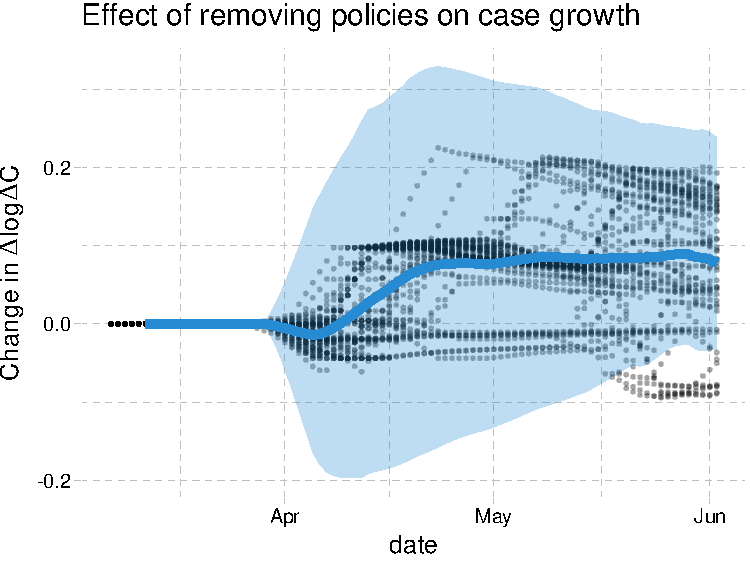
\includegraphics[width=0.45\textwidth]{../tables_and_figures/us-nop-dgrowth}
    &
      \includegraphics[width=0.45\textwidth]{../tables_and_figures/us-nop-rel}\\

 %  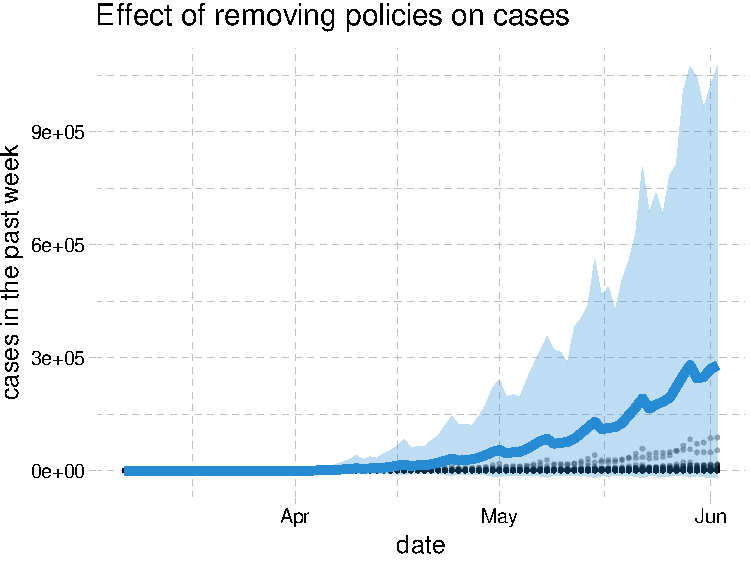
\includegraphics[width=0.45\textwidth]{tables_and_figures/us-nop-dcases}
      %  \includegraphics[width=0.45\textwidth]{tables_and_figures/us-nop-dgrowth_deaths}
    \end{tabular}
  \end{minipage}
\end{figure}

\begin{figure}[ht]
 % \caption{Effect of removing policies on deaths: national average \label{fig:US-nop-ddeaths}}
  \begin{minipage}{\linewidth}
    \centering
    \begin{tabular}{cc}
    \includegraphics[width=0.45\textwidth]{../tables_and_figures/us-nop-dgrowth_deaths}
      &
      \includegraphics[width=0.45\textwidth]{../tables_and_figures/us-nop-rel_deaths}\\

  %  \includegraphics[width=0.45\textwidth]{tables_and_figures/us-nop-dcases_deaths}
      %  \includegraphics[width=0.45\textwidth]{tables_and_figures/us-nop-rel}
    \end{tabular}
  \end{minipage}
\end{figure}

\end{frame}
%----------------------------------------------------------------------------------------%




%----------------------------------------------------------------------------------------%

\begin{frame}
  \frametitle{Conclusion }

\begin{itemize}
\item  A useful SEM framework to estimate the roles of policies and information on determining the spread of Covid-19. \smallskip
 
\item  If US-wide mask mandates had been adopted on April 1st, as much as 40\% (17\% - 55\%) lives could have been saved.\smallskip

\item Keeping non-essential businesses open would have lead to  -20\% to 40\% increase in deaths.\smallskip

\item Not having implemented any policy could have led to\qquad  [0,  10] fold increase in deaths.  % (intersecting confidence intervals for relative increase in cases and death).


\end{itemize}
 

\end{frame}
%----------------------------------------------------------------------------------------%


%----------------------------------------------------------------------------------------%

\begin{frame}
  \frametitle{Conclusion}
  
\begin{itemize}
  
\item People voluntarily reduce their mobility in response to a higher number of cases and deaths.\smallskip

 
\item There is much ambiguity related to the total effect of policies vs voluntary behavior, which can not be identified well from the US data. \smallskip

\item Closure of schools has potentially large effects via behavior, keeping people at home, but school policy has almost no cross-sectional variation.\smallskip % Including national cases as information reduces the estimated school effect, resulting in greater attribution to behavior.\smallskip


%\item To Do: feedback effect from information on national cases/deaths.
  
\end{itemize}
  
\end{frame}
%----------------------------------------------------------------------------------------%



\begin{frame}[allowframebreaks]
\frametitle{Bibliography}
%\large
\footnotesize
\bibliography{../covid}
\end{frame}


>>>>>>> counterfactuals
%----------------------------------------------------------------------------------------%

\begin{frame}
  \frametitle{Correlations between policies and behavior variables}\vspace{-0.05cm}
\begin{table}%\caption{Correlations among Policies and Behavior \label{tab:correlation}}\vspace{-0.2cm}
  \begin{minipage}{\linewidth}
    \resizebox{\linewidth}{!}{
      
\begin{tabular}{lccccccccccc}
\toprule
\rotatebox{90}{ } & \rotatebox{90}{workplaces} & \rotatebox{90}{retail} & \rotatebox{90}{grocery} & \rotatebox{90}{transit} & \rotatebox{90}{masks for employees} & \rotatebox{90}{closed K-12 schools} & \rotatebox{90}{stay at home} & \rotatebox{90}{closed movie theaters} & \rotatebox{90}{closed restaurants} & \rotatebox{90}{closed non-essent bus} & \rotatebox{90}{business closure policies}\\
\midrule
workplaces & 1.00 &  &  &  &  &  &  &  &  &  & \\
retail & 0.93 & 1.00 &  &  &  &  &  &  &  &  & \\
grocery & 0.75 & 0.83 & 1.00 &  &  &  &  &  &  &  & \\
transit & 0.89 & 0.92 & 0.83 & 1.00 &  &  &  &  &  &  & \\
masks for employees & -0.32 & -0.17 & -0.15 & -0.29 & 1.00 &  &  &  &  &  & \\
\addlinespace
closed K-12 schools & -0.91 & -0.79 & -0.55 & -0.72 & 0.43 & 1.00 &  &  &  &  & \\
stay at home & -0.69 & -0.69 & -0.70 & -0.71 & 0.28 & 0.62 & 1.00 &  &  &  & \\
closed movie theaters & -0.81 & -0.76 & -0.64 & -0.71 & 0.34 & 0.82 & 0.72 & 1.00 &  &  & \\
closed restaurants & -0.77 & -0.82 & -0.68 & -0.76 & 0.21 & 0.74 & 0.72 & 0.82 & 1.00 &  & \\
closed non-essent bus & -0.65 & -0.68 & -0.68 & -0.64 & 0.08 & 0.56 & 0.76 & 0.68 & 0.71 & 1.00 & \\
\addlinespace
business closure policies & -0.84 & -0.84 & -0.75 & -0.79 & 0.24 & 0.78 & 0.81 & 0.92 & 0.93 & 0.87 & 1.00\\
\bottomrule
\end{tabular}
    }\smallskip
%       \begin{flushleft}
%         \scriptsize
%         Each off-diagonal entry reports a correlation coefficient of
%         a pair of policy and behavior variables.
%       \end{flushleft}
  \end{minipage}
\end{table}
<<<<<<< HEAD
 
=======

>>>>>>> counterfactuals
\end{frame}
%----------------------------------------------------------------------------------------%




<<<<<<< HEAD



%----------------------------------------------------------------------------------------%

\begin{frame}
  \frametitle{The Effect of Policies and Information on Behavior}

% We first examine how policies and information affect social distancing behaviors by estimating a version of (\ref{eq:R2}):
\begin{align}
  {\bcolor B_{it}^j}
  %& = {\pcolor (\beta^j)' P_{it} }  + {\icolor \gamma_{1}^j \log(t) + \gamma_{2}^j \log (\Delta C_{i,t-14}) +  \gamma_{3}^j Y_{i,t-7}} + {\wcolor (\delta_B^j)' W_{it}} + \varepsilon_{it}^j \nonumber\\
  & = {\pcolor (\beta^j)' P_{it}} + {\icolor (\gamma^j)' I_{it}} +
    {\wcolor (\delta_B^j)' W_{it}} + \varepsilon_{it}^{bj}, \notag
\end{align}

\begin{itemize}
\item   ${\bcolor B_{it}^j}$:  ``Transit,''  ``Workplaces''  ``Grocery," and ``Retail'' from Google Mobility Reports,\smallskip
\item  $ {\pcolor  P_{it}} $: masks for employees, stay at home, closure of schools, closure of movie theaters, closure of non-essential businesses.\smallskip
\item $ {\icolor I_{it}} $: past growth of cases/deaths, the log of past cases/deaths, national-level cases/deaths and their growth.\smallskip
\item $ {\wcolor   W_{it}}$: state-level characteristics   and month dummies.
=======
%----------------------------------------------------------------------------------------%

\begin{frame}
  \frametitle{Counterfactual Experiments}

\begin{itemize}
\item
Set initial \(\Delta \log \Delta D\) and
\(\log \Delta D\)  to their first observed values. \smallskip
\item  Other regressors at their observed
values. \smallskip
\item Error terms are drawn with replacement from the residuals.\smallskip
\item Do this many times and report the average over draws of the
residuals to obtain counterfactual results.   \smallskip

\item To obtain a point-wise 90\% confidence interval, we repeat the above with
coefficients drawn randomly from their asymptotic distribution.


>>>>>>> counterfactuals
\end{itemize}


\end{frame}
%----------------------------------------------------------------------------------------%


<<<<<<< HEAD

\begin{frame}[allowframebreaks]
\frametitle{Bibliography}
%\large
\footnotesize
\bibliography{../covid}
\end{frame}


 
\end{document}

  
=======
%----------------------------------------------------------------------------------------%

\begin{frame}
  \frametitle{SIR Model and Empirical Specification}\vspace{-0.05cm}

 SIR Model with confirmed cases $ \dot{C}(t)$ and testing $\tau(t)$:
\begin{align*}
  \dot{S}(t)  = -\frac{S(t)}{N} \beta(t) \Infected(t),\qquad
 & \dot{\Infected}(t)   = \frac{S(t)}{N} \beta(t) \Infected(t) - \gamma  \Infected(t), \\
  % \frac{S(t-\ell)}{N} \beta(t-\ell)  \Infected(t-\ell) \label{eq:i} \\
  \dot{\Recovered}(t)   = (1-\kappa) \gamma  \Infected(t),\qquad %  \frac{S(t-\ell)}{N} \beta(t-\ell)    \Infected(t-\ell) \label{eq:r} \\
 &  \dot{D}(t) = \kappa \gamma \Infected(t), %  \frac{S(t-\ell)}{N} \beta(t-\ell)   \Infected(t-\ell)
\qquad \dot{C}(t) = \tau(t) \Infected(t). \qquad
\end{align*}


  Differentiating  { $\dot{C}(t) = \tau(t) \Infected(t)$},
  \begin{align*}
    \frac{\ddot{C}(t)}{\dot{C}(t)}
              & =
                \frac{S(t)}{N} \beta(t) -\gamma  + \frac{\dot{\tau}(t)}{\tau(t)}.
                \end{align*}
       Discrete-time analogue with $\frac{S(t)}{N} \beta(t)\approx  X_{it}' \theta + \epsilon_{it}$:\medskip
   \begin{align*}
 {\ycolor Y_{it} }:=   {\ycolor \Delta \log \Delta C_{it}}    = X_{it}' \theta + \epsilon_{it} - \gamma+\delta_T {\wcolor \Delta
      \log(T)_{it}}.
                 \end{align*}



\end{frame}

%----------------------------------------------------------------------------------------%


\end{document}
	
>>>>>>> counterfactuals
